\clearpage
\chapter*{ՀԱՎԵԼՎԱԾ 2. ՆԱԽԱԳԾԱՅԻՆ ԵՎ ՃԱՐՏԱՐԱՊԵՏԱԿԱՆ ՆՅՈՒԹԵՐ}
\addcontentsline{toc}{chapter}{ՀԱՎԵԼՎԱԾ 2. ՆԱԽԱԳԾԱՅԻՆ ԵՎ ՃԱՐՏԱՐԱՊԵՏԱԿԱՆ ՆՅՈՒԹԵՐ}
\setcounter{figure}{0}
\renewcommand{\thefigure}{2.\number\value{figure}}
\sloppy

Այս հավելվածում ներկայացված են նախագծային նյութերը՝ արդեն տեսանելի սխեմաների և wireframe-երի տեսքով։ Դրանք լրացնում են Հավելված 1-ում ներկայացված էկրանապատկերները. եթե էկրանապատկերները ցույց են տալիս համակարգի վերջնական տեսքը, ապա այս սխեմաները ցույց են տալիս այն նախագծային տրամաբանությունը, որով համակարգը ձևավորվել է՝ խնդիրներից և մեթոդներից դեպի ծրագրային արդյունք անցումը փաստաթղթավորելու համար։

\begin{figure}[h]
  \centering
  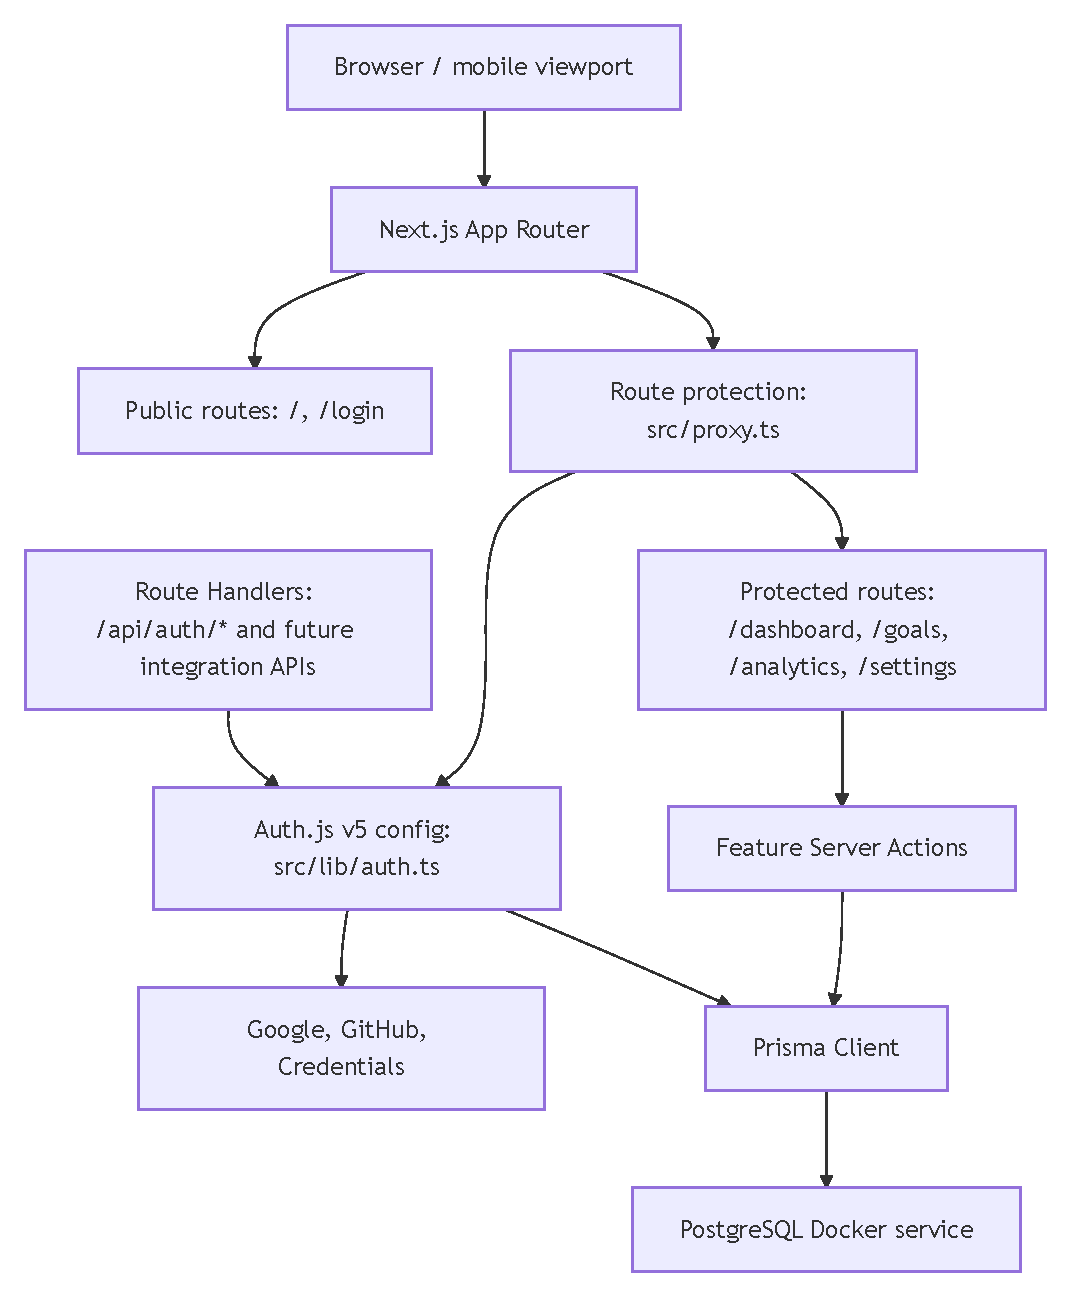
\includegraphics[width=\textwidth,height=0.78\textheight,keepaspectratio]{figures/rendered/app-architecture.pdf}
  \caption{Հավելվածի ընդհանուր ճարտարապետությունը՝ Next.js App Router, Auth.js, server actions, Prisma և PostgreSQL շերտերով}
  \label{fig:appendix-app-architecture}
\end{figure}

\clearpage
\begin{figure}[h]
  \centering
  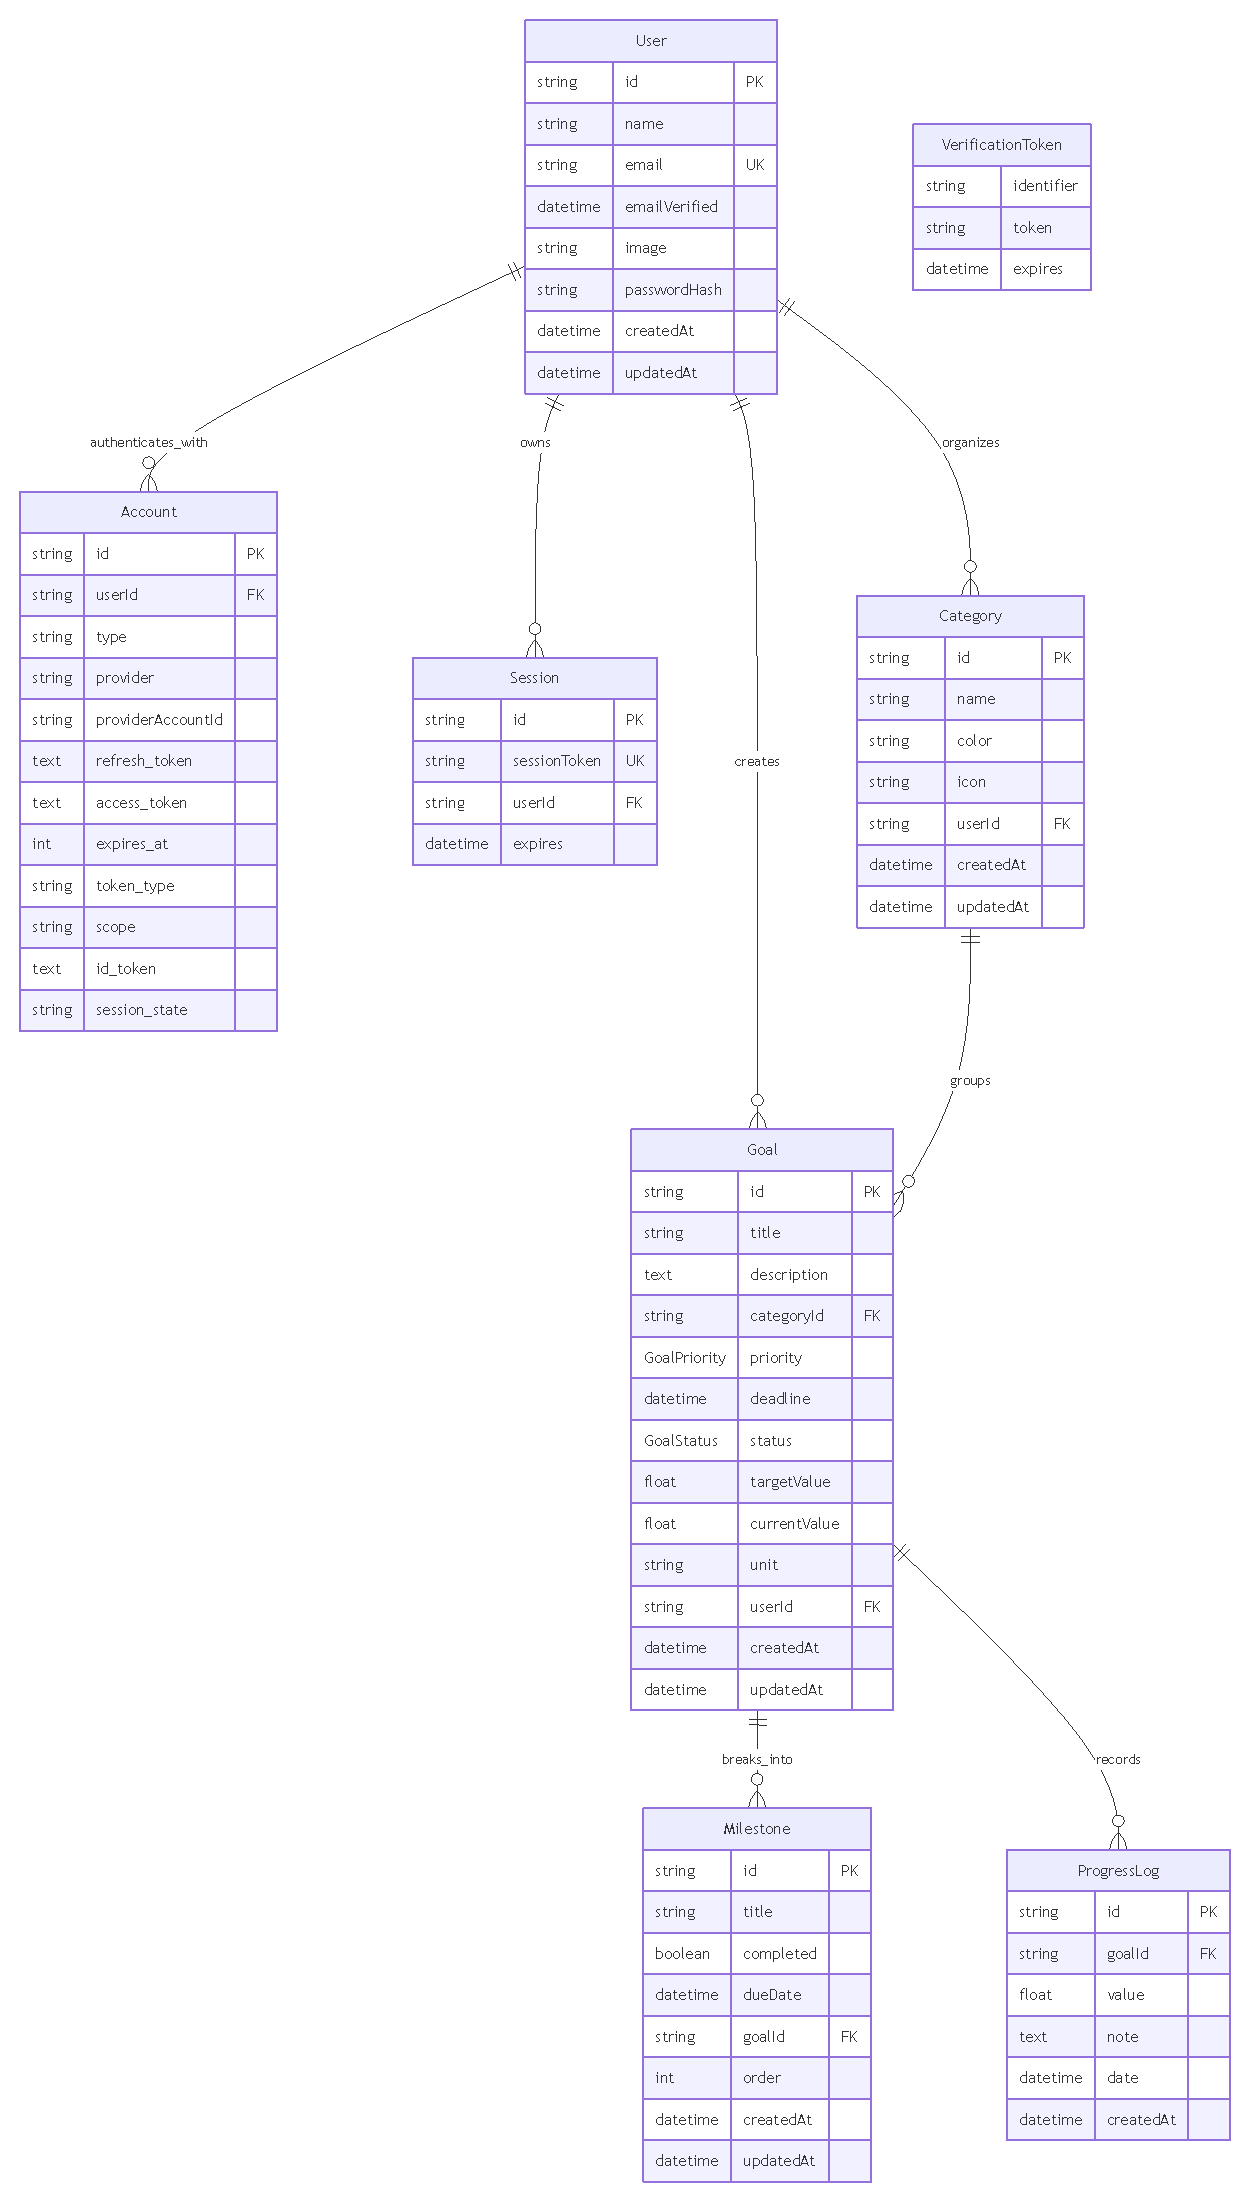
\includegraphics[width=\textwidth,height=0.82\textheight,keepaspectratio]{figures/rendered/er-diagram.pdf}
  \caption{Տվյալների բազայի ER սխեման՝ օգտատերերի, նպատակների, կատեգորիաների, ենթանպատակների և առաջընթացի գրառումների կապերով}
  \label{fig:appendix-er-diagram}
\end{figure}

\clearpage
\begin{figure}[h]
  \centering
  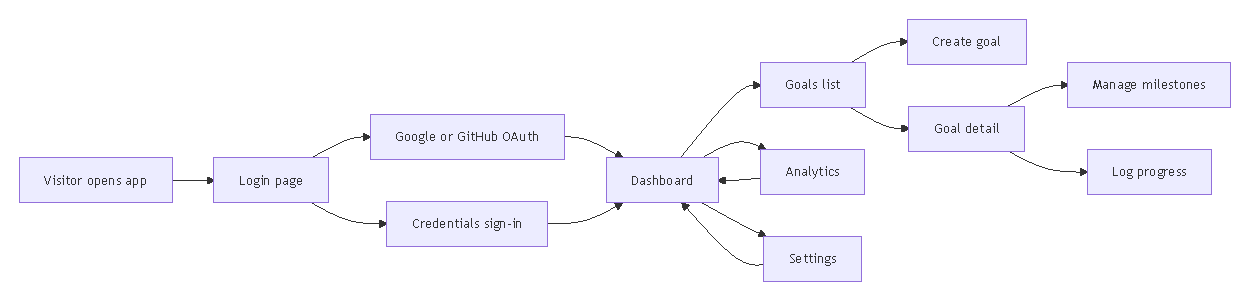
\includegraphics[width=\textwidth,height=0.55\textheight,keepaspectratio]{figures/rendered/user-flow.pdf}
  \caption{Օգտատիրոջ հիմնական հոսքը՝ մուտքից դեպի dashboard, նպատակների կառավարում, analytics և settings էջեր}
  \label{fig:appendix-user-flow}
\end{figure}

\begin{figure}[h]
  \centering
  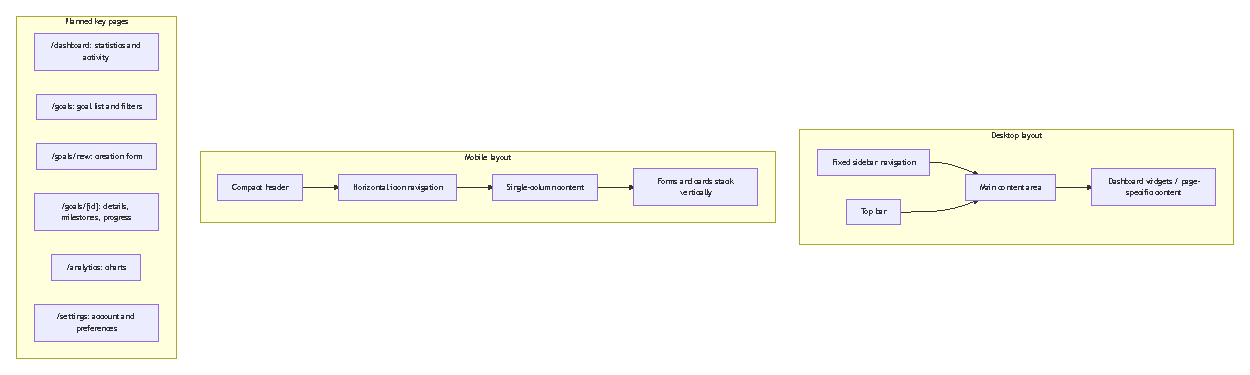
\includegraphics[width=\textwidth,height=0.55\textheight,keepaspectratio]{figures/rendered/wireframes.pdf}
  \caption{Desktop և mobile wireframe-երը՝ հիմնական էջերի կառուցվածքային պլանով}
  \label{fig:appendix-wireframes}
\end{figure}
\fussy
